% TIP: keep track of what each package does with a commented line after the load package command for the package - the packages build up quickly

\documentclass{beamer} % for more information on beamer see: https://www.sharelatex.com/learn/Beamer

\usetheme{CambridgeUS} % see http://deic.uab.es/~iblanes/beamer_gallery/ for many others

\usepackage{graphicx} % Necessary for inserting graphics

% For citations - here using Chicago style
\usepackage[utf8]{inputenc}
\usepackage[authordate-trad,backend=biber]{biblatex-chicago} 
\addbibresource{MyLibrary.bib} % Specify where your .bib file (from Zotero!) is

% Three packages for nice tables and figures
\usepackage{booktabs}
\usepackage{dcolumn} 
\usepackage{wrapfig} 
\usepackage{subfig} % For multiple figures side-by-side

% unlike the document article class, you specify title prior to opening the document
\title{Basic LaTeX beamer demonstration file}
\subtitle{CSDC Methods Winter School}
\author{Aengus Bridgman}

\begin{document}

\frame{\titlepage} % Add a title page

\section{Introduction} % Add a section title - functionality varies by theme

% each page/slide begins and ends with a frame, that you then give a title
\begin{frame}
\frametitle{Using Beamer}

\begin{itemize} % For bullet points
  \item LaTeX Beamer and article documentclass have very similar functionality
    \begin{enumerate} % For list of items
      \item Can do lists
      \item Can input tables
      \item Can input plots
      \item Can do bibliographies and citations: \parencite*{fox_package_2017}
    \end{enumerate}
\end{itemize}

\end{frame}

\section{Findings}

% each slide begins with a frame
\begin{frame}
\frametitle{Plots}

\begin{figure}[h]
  \centering
  \subfloat[Plot 1]{{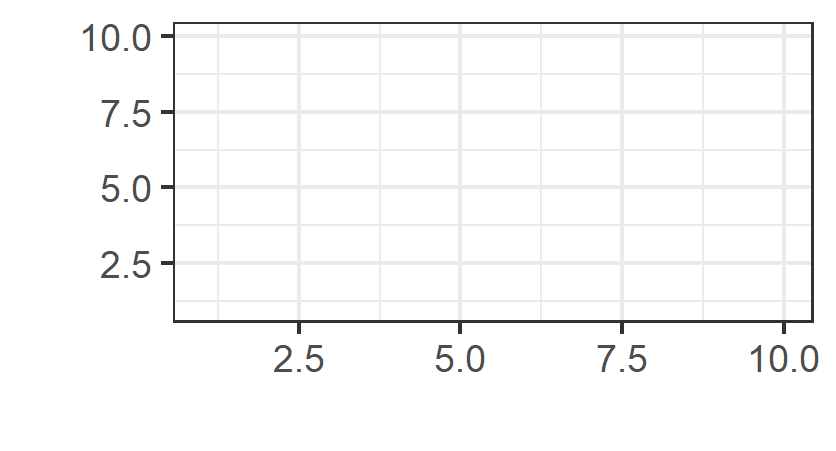
\includegraphics[width=5cm]{plot.png} }}
  \qquad
  \subfloat[Plot 2]{{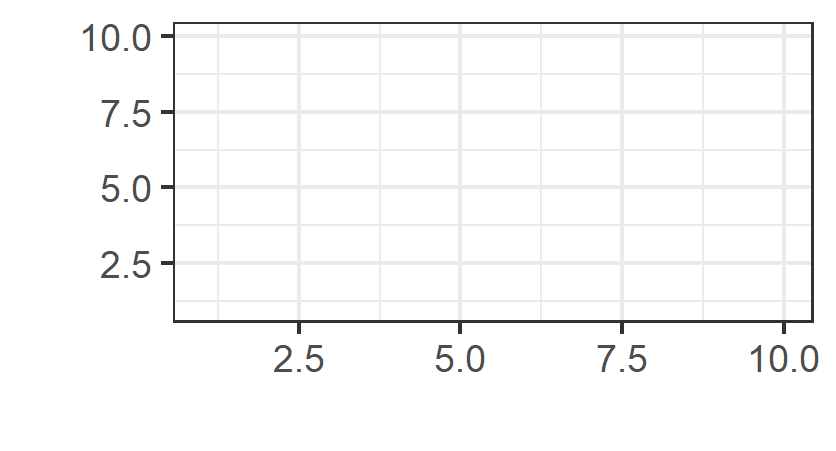
\includegraphics[width=5cm]{plot.png} }}
  \caption{Two plots side by side}
\end{figure}

\end{frame}

\begin{frame}
	\frametitle{Tables}
    %latex.default(ownership_df, caption = "Perceptions of issue ownership for partisans in Canada for the 2015 federal elections",     label = "partisanownership", booktabs = TRUE, title = "",     cgroup = c("", "Liberal", "Conservative", "NDP"), n.cgroup = c(1,         2, 2, 2), colheads = c("Issue", "Own", "Dif", "Own",         "Dif", "Own", "Dif"), file = paste(save_location, "partisanownership.tex",         sep = ""))%
\begin{table}[!ht]
\caption{Perceptions of issue ownership for partisans in Canada for the 2015 federal elections\label{partisanownership}} 
\begin{center}
\begin{tabular}{llcrrcrrcrr}
\toprule
\multicolumn{1}{l}{\bfseries }&\multicolumn{1}{c}{\bfseries }&\multicolumn{1}{c}{\bfseries }&\multicolumn{2}{c}{\bfseries Liberal}&\multicolumn{1}{c}{\bfseries }&\multicolumn{2}{c}{\bfseries Conservative}&\multicolumn{1}{c}{\bfseries }&\multicolumn{2}{c}{\bfseries NDP}\tabularnewline
\cline{4-5} \cline{7-8} \cline{10-11}
\multicolumn{1}{l}{}&\multicolumn{1}{c}{Issue}&\multicolumn{1}{c}{}&\multicolumn{1}{c}{Own}&\multicolumn{1}{c}{Dif}&\multicolumn{1}{c}{}&\multicolumn{1}{c}{Own}&\multicolumn{1}{c}{Dif}&\multicolumn{1}{c}{}&\multicolumn{1}{c}{Own}&\multicolumn{1}{c}{Dif}\tabularnewline
\midrule
1&Crime&&$54.5$&$22.2$&&$66.2$&$10.5$&&$36.3$&$39.2$\tabularnewline
2&Environment&&$44.0$&$36.9$&&$32.6$&$42.2$&&$32.8$&$50.5$\tabularnewline
3&Defence&&$52.9$&$24.0$&&$68.8$&$ 8.1$&&$29.0$&$45.3$\tabularnewline
4&Immigration&&$64.6$&$12.1$&&$49.6$&$23.5$&&$44.0$&$30.9$\tabularnewline
\bottomrule
\end{tabular}\end{center}
\end{table}

\end{frame}

% Like R, compiling .tex files sometimes produces non-fatal warning messages. In this case, it is biblatex trying to use another non-functional package. You can filter these out (see https://tex.stackexchange.com/questions/202988/beamer-patching-footnotes-warning-patching-footnotes-failed-footnote-detectio) or just ignore them. 

\end{document}